% !TEX option = --shell-escape

\documentclass{beamer}


\usepackage{tikz}

% GNUPLOT required



\begin{document}

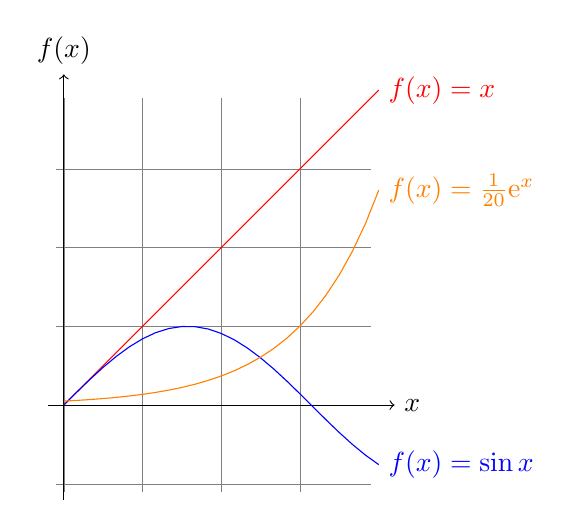
\begin{tikzpicture}[domain=0:4]
    \draw[very thin,color=gray] (-0.1,-1.1) grid (3.9,3.9);
    \draw[->] (-0.2,0) -- (4.2,0) node[right] {$x$};
    \draw[->] (0,-1.2) -- (0,4.2) node[above] {$f(x)$};
    \draw[color=red,domain=0:4] plot (\x,{\x}) 
        node[right] {$f(x) = x$};
    \draw[color=blue,domain=0:4] plot (\x,{sin(\x r)}) 
        node[right] {$f(x) = \sin x$};
    \draw[color=orange,domain=0:4] plot (\x,{0.05*exp(\x)}) 
        node[right] {$f(x) = \frac{1}{20} \mathrm e^x$};
\end{tikzpicture}

testing
\end{document}